\documentclass[11pt,a4paper]{article}

% ---------------------------------------------------------------------------
% ThreatInt — engineering build report ("how it was built")
% Companion to threatint_report.tex (the technical research report).
% ---------------------------------------------------------------------------
\usepackage[T1]{fontenc}
\usepackage[utf8]{inputenc}
\usepackage{lmodern}
\usepackage[margin=2.2cm,top=2.6cm,bottom=2.4cm]{geometry}
\usepackage{graphicx}
\usepackage{booktabs}
\usepackage{array}
\usepackage{tabularx}
\usepackage{colortbl}
\usepackage{xcolor}
\usepackage{titlesec}
\usepackage{fancyhdr}
\usepackage{enumitem}
\usepackage{amsmath}
\usepackage{caption}
\usepackage{tcolorbox}
\usepackage{listings}
\usepackage[hidelinks]{hyperref}
\tcbuselibrary{skins,breakable}

\definecolor{navy}{HTML}{1B3A5C}
\definecolor{steel}{HTML}{34668C}
\definecolor{sky}{HTML}{5B9BD5}
\definecolor{crimson}{HTML}{C0392B}
\definecolor{amber}{HTML}{E08A1E}
\definecolor{forest}{HTML}{2E8B57}
\definecolor{grey}{HTML}{8A99A8}
\definecolor{paper}{HTML}{F7F9FB}
\definecolor{ink}{HTML}{1D2733}
\definecolor{purple}{HTML}{6B4C9A}

\titleformat{\section}{\normalfont\Large\bfseries\color{navy}}{\thesection}{0.7em}{}
\titleformat{\subsection}{\normalfont\large\bfseries\color{steel}}{\thesubsection}{0.6em}{}
\titleformat{\subsubsection}{\normalfont\normalsize\bfseries\color{ink}}{\thesubsubsection}{0.5em}{}
\titlespacing*{\section}{0pt}{1.4em}{0.6em}

\pagestyle{fancy}
\fancyhf{}
\renewcommand{\headrulewidth}{0.4pt}
\fancyhead[L]{\footnotesize\color{grey}ThreatInt --- Engineering Build Report}
\fancyhead[R]{\footnotesize\color{grey}\thepage}
\captionsetup{font=small,labelfont={bf,color=navy},justification=centering}

\newtcolorbox{keybox}[1][]{
  colback=paper, colframe=steel, boxrule=0.8pt, arc=2pt,
  left=8pt, right=8pt, top=6pt, bottom=6pt, breakable,
  fonttitle=\bfseries\color{white}, coltitle=white, colbacktitle=steel, title=#1}
\newtcolorbox{lessonbox}[1][]{
  colback=forest!6, colframe=forest, boxrule=0.7pt, arc=2pt,
  left=8pt, right=8pt, top=6pt, bottom=6pt, breakable,
  fonttitle=\bfseries\color{white}, coltitle=white, colbacktitle=forest, title=#1}
\newtcolorbox{warstory}[1][]{
  colback=crimson!5, colframe=crimson, boxrule=0.7pt, arc=2pt,
  left=8pt, right=8pt, top=6pt, bottom=6pt, breakable,
  fonttitle=\bfseries\color{white}, coltitle=white, colbacktitle=crimson, title=#1}

\lstset{
  basicstyle=\ttfamily\footnotesize, backgroundcolor=\color{paper},
  frame=single, rulecolor=\color{grey!50},
  keywordstyle=\color{steel}\bfseries, stringstyle=\color{forest},
  commentstyle=\color{grey}\itshape,
  numbers=left, numberstyle=\tiny\color{grey}, numbersep=8pt,
  breaklines=true, showstringspaces=false, columns=fullflexible, keepspaces=true,
  xleftmargin=14pt, framexleftmargin=12pt,
}
\newcommand{\code}[1]{\texttt{\small #1}}

% ---------------------------------------------------------------------------
\begin{document}

% ============================== TITLE PAGE =================================
\begin{titlepage}
\pagecolor{purple}
\color{white}
\centering
\vspace*{3.2cm}
{\fontsize{15}{18}\selectfont\color{white!80}\textsc{Engineering Build Report}}\\[0.8cm]
{\fontsize{40}{46}\selectfont\bfseries How I Built ThreatInt}\\[0.5cm]
{\fontsize{16}{20}\selectfont\color{white!88}
From a one-paragraph README to a tested,\\ deployed, documented threat-intelligence pipeline}\\[2.2cm]
\rule{11cm}{0.6pt}\\[0.8cm]
{\fontsize{12}{15}\selectfont\color{white!85}
\textbf{Repository:} \texttt{Ashwin-kumar-jonjale/ThreatInt}\\[0.3cm]
\textbf{Branch:} \texttt{feat/threat-intel-pipeline} · HEAD \texttt{34f68b4}\\[0.3cm]
\textbf{Duration:} 3 days · 5 commits · 2{,}246 lines of source\\[0.3cm]
\textbf{Result:} 60 tests passing · pyflakes clean · 3 deploy targets}
\vfill
{\fontsize{10}{13}\selectfont\color{white!65}
Companion to the \emph{Technical Research Report}. This document is the build
log: the decisions, the workflow, the obstacles, and what I would change.\\[0.4cm]
\LaTeX{} · \today}
\end{titlepage}
\pagecolor{white}
\color{ink}

% ============================== TOC ========================================
\pagenumbering{roman}
\tableofcontents
\newpage
\pagenumbering{arabic}

% ============================== 1. PROLOGUE ================================
\section{Prologue: what I started with}

The repository began as almost nothing. The entire initial commit
(\texttt{d6ce7ce}) was a single file containing three lines --- a README whose
whole content was a problem statement:

\begin{quote}\itshape
``Security analysts manually cross-check hundreds of threat alerts daily, a slow
and error-prone process. Built a pipeline that automatically collects threat
intelligence data (malicious IPs, domains, URLs) from multiple trusted sources,
cross-verifies reliability, and applies machine learning to classify malicious
indicators and cluster related threats into attack campaigns, reducing manual
analyst workload.''
\end{quote}

That was the brief, the specification, and the entire codebase. Everything else
--- 2{,}246 lines of source, 679 lines of tests, a web dashboard, three
deployment paths and two PDF reports --- was built on top of it. This report
describes how.

\begin{keybox}[The brief --- decomposed]
The one paragraph hides four deliverables and one implicit constraint:
\begin{enumerate}[leftmargin=1.3em,itemsep=1pt,topsep=2pt]
  \item \textbf{Collect} from multiple trusted sources $\rightarrow$ a pluggable collector layer.
  \item \textbf{Cross-verify reliability} $\rightarrow$ per-source trust scoring, not a flat union.
  \item \textbf{Classify with ML} $\rightarrow$ a supervised model over engineered features.
  \item \textbf{Cluster into campaigns} $\rightarrow$ unsupervised grouping of related indicators.
  \item \emph{(implicit)} \textbf{Reduce analyst workload} $\rightarrow$ the output must be usable, not a dump.
\end{enumerate}
\end{keybox}

% ============================== 2. APPROACH ================================
\section{How I framed the work}

Before writing code I made one decision that shaped everything else: I treated
the implicit fifth requirement as the real one. A pipeline that collects and
classifies but produces an unreadable wall of JSON has not reduced anyone's
workload. So from the first commit I built toward three \emph{surfaces} for the
same data: a CLI for batch runs, machine-readable exports for integration, and
eventually a dashboard for humans. That is why the project has a presentation
layer at all --- it was not an afterthought.

I also committed early to two properties that made the rest of the work
verifiable:

\begin{itemize}[leftmargin=1.4em,itemsep=3pt]
  \item \textbf{Determinism.} A single \code{random\_seed} governs every
    stochastic step. This means any number I report can be reproduced by anyone
    running the same command --- which is what let me write a metrics-backed
    research report at all.
  \item \textbf{Network-optional operation.} Every collector can read a bundled
    fixture. This meant the pipeline ran identically on a laptop, in CI, and in
    a container, with no API keys and no flakiness.
\end{itemize}

\subsection{The plan}
I broke the work into four increments, each independently shippable and
testable, and built them in order:

\begin{center}
\begin{tabularx}{\linewidth}{@{}>{\bfseries}p{1.4cm}>{\bfseries}p{4.4cm}X@{}}
\toprule
\rowcolor{paper}\textbf{Phase} & \textbf{Deliverable} & \textbf{Definition of done} \\
\midrule
1 & Core pipeline & \code{threatint} runs end to end offline; tests pass. \\
2 & Web dashboard & Flask console serves the same results live. \\
3 & Deployable & Static export + Docker + CI; runs with no server. \\
4 & Documentation & README, AGENTS.md and a research report with real metrics. \\
\bottomrule
\end{tabularx}
\end{center}

\begin{figure}[htbp]
\centering
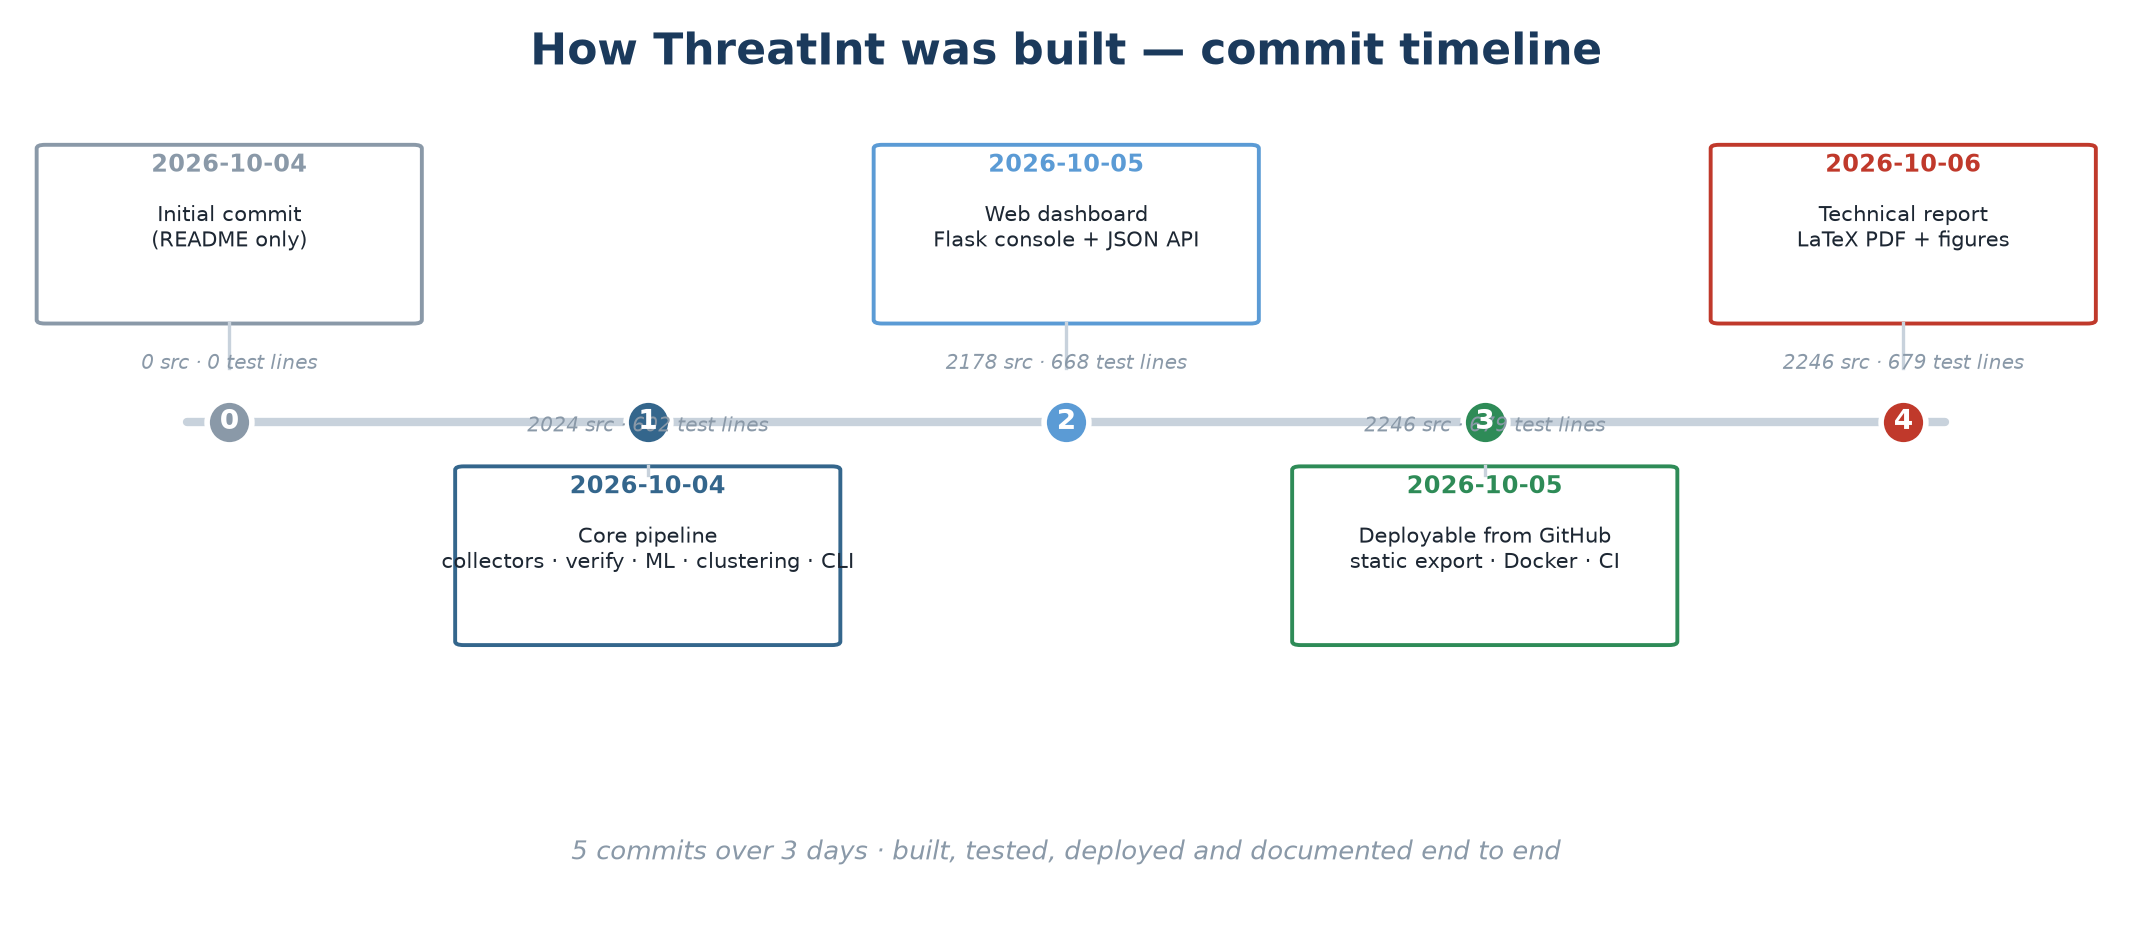
\includegraphics[width=\linewidth]{figures/figB1_timeline.png}
\caption{The build timeline reconstructed from git history. Five commits over
three days; the core pipeline (commit 1) carried the bulk of the design work,
with each later commit adding a surface without touching the core.}
\label{fig:timeline}
\end{figure}

% ============================== 3. PHASE 1 =================================
\section{Phase 1 --- the core pipeline}

This was the largest single commit: 35 files and roughly 2{,}000 lines of source
and tests. I wrote it in dependency order, bottom-up, so each layer could be
tested before the layer above it existed.

\subsection{Order of construction}
\begin{enumerate}[leftmargin=1.4em,itemsep=3pt]
  \item \textbf{The data model first} (\code{models.py}). I defined
    \code{RawRecord}, \code{Observation}, \code{Indicator}, \code{Campaign} and
    \code{SourceReliability} as plain dataclasses before any logic. Getting the
    \emph{shapes} right first meant every later module had a stable contract to
    code against, and the whole pipeline became a clean sequence of transforms
    between them.
  \item \textbf{Normalisation} (\code{normalize.py}). Feeds are messy, so I
    built refanging, type detection and canonicalisation before collectors ---
    the collectors depend on it, not the reverse.
  \item \textbf{Collectors} (\code{collectors/base.py}). One abstract base with
    the shared parsing helpers, two concrete collectors (HTTP and offline), and
    a factory. The fixture fallback lives here.
  \item \textbf{Cross-verification} (\code{verification/}). The analytical
    core: source reliability and indicator scoring. This was the hardest part to
    get right and the part I rewrote the most.
  \item \textbf{Features, classifier, clustering.} With clean, deduplicated,
    scored indicators in hand, the ML layer was straightforward to bolt on.
  \item \textbf{Orchestration, reporting, CLI.} Finally, tie it together and
    expose it.
\end{enumerate}

\subsection{The decisions that mattered}
Three design choices in Phase 1 had outsized consequences.

\subsubsection{Identity by hash, not by counter}
An indicator's ID is \code{sha256("type:value")[:16]}. This was a small line of
code with a large payoff: the same observable reported by five different feeds
collapses to one object with \emph{no coordination between collectors}, and the
ID is stable across runs. That stability later let campaign IDs --- themselves
hashes of member IDs --- be reproducible too, which is a genuinely useful
operational property I did not fully appreciate until the clustering phase.

\subsubsection{Trust as a computed quantity}
The naive approach is to union all feeds and trust everything. I rejected that
immediately because it ignores the brief's word \emph{reliability}. Instead,
each feed gets a static analyst prior that is \emph{blended} with dynamic
signals measured against the cross-source consensus: precision, recall and mean
pairwise Jaccard agreement. A volume-damping factor stops a feed with three
reports from swinging wildly. The result (from the reference run) is that a
low-prior feed with excellent measured behaviour can outrank a high-prior feed
with a noisy batch --- exactly the behaviour the brief asked for.

\subsubsection{Fail soft, per source}
Collection is wrapped per-collector and \code{HttpCollector} catches broadly and
falls back to its fixture. This is the single most valuable robustness decision
in the codebase. It was validated later when a live run hit an HTTP 403 on one
endpoint and 32{,}289 records on another, and completed cleanly anyway.

\begin{lessonbox}[Lesson: build the offline path first]
Making fixtures a first-class citizen, not a testing afterthought, is what made
the pipeline testable, CI-friendly, deterministic \emph{and} resilient. It cost
a little extra design up front and paid for itself many times over.
\end{lessonbox}

% ============================== 4. PHASE 2 =================================
\section{Phase 2 --- the web dashboard}

With the pipeline producing structured results, the dashboard was a thin
read-only layer over them (commit \texttt{2b28b2e}, 8 files). The design
constraint was deliberate: \textbf{the pipeline must not be remotely
reconfigurable}. The web layer accepts only pagination and filter parameters,
and all indicator text is escaped client-side. This kept the security surface
tiny.

The console presents four things an analyst actually needs: summary cards, a
filterable indicator table (probability, verdict, type, source count,
reliability, campaign), a campaign grid, and a source-reliability ranking. I
also added a small but important touch: \textbf{every indicator is defanged
before display} (\code{hxxp://\dots[.]}), so a live IOC is never a clickable
link in a browser.

\subsection{Testing a web layer without a browser}
I tested the Flask app with its real test client rather than mocks --- hitting
\code{/healthz}, the JSON endpoints, and the pagination/filter logic directly.
This caught a subtle bug class early: malformed \code{limit}/\code{offset}
values needed to fall back to safe defaults rather than raising.

% ============================== 5. PHASE 3 =================================
\section{Phase 3 --- making it deployable from GitHub}

This phase (commit \texttt{7dd9e19}) came from a follow-up request: ``deploy it
from GitHub, or make it deployable from the GitHub itself.'' That phrasing
pushed me toward the strongest interpretation --- the repository should be able
to produce a working deployment with no server and no secrets.

\subsection{The dual-mode template}
The key move was to make the dashboard template work in \emph{two} modes: live
(consuming the Flask JSON API) and static (data inlined, filtering and
pagination done client-side in JavaScript). One template, two data paths. This
guarantees the hosted static artifact and the live server cannot drift apart,
because they render the same file.

\subsection{The static exporter}
\code{static\_export.py} runs the pipeline and writes a single self-contained
\code{index.html} with the entire result set inlined (about 131\,KB). No build
step, no bundler, no server --- a file you can open directly or host anywhere.

\subsection{Three deployment paths}
\begin{center}
\begin{tabularx}{\linewidth}{@{}>{\bfseries}p{3.5cm}X@{}}
\toprule
\rowcolor{paper}\textbf{Target} & \textbf{Mechanism} \\
\midrule
GitHub Pages & \code{publish-dashboard.yml} renders the static console and publishes it on push to \code{main}. \\
Docker & A \code{Dockerfile} installs the package, bakes the static dashboard into the image and serves the live console. \\
CI & \code{ci.yml} runs \code{pyflakes} and the full test suite on two Python versions. \\
\bottomrule
\end{tabularx}
\end{center}

\begin{warstory}[War story: the Docker daemon]
The container image built and served correctly, but only after discovering the
Docker daemon was present but \emph{not running} by default in the environment,
and needed to be started manually first. A small thing, but exactly the kind of
assumption that breaks a ``it works on my machine'' deployment. Worth recording
so the next person does not lose the same half hour.
\end{warstory}

% ============================== 6. PHASE 4 =================================
\section{Phase 4 --- documenting with real numbers}

The final phase (commit \texttt{34f68b4}) was the technical research report. The
guiding rule was that \textbf{every number must come from a real run}. Rather
than describe the system in prose and hand-wave at performance, I:

\begin{enumerate}[leftmargin=1.4em,itemsep=3pt]
  \item ran the pipeline offline and dumped the results to
    \code{report/data/result.json};
  \item wrote \code{make\_figures.py} to build every chart \emph{from that
    JSON}, so no figure can disagree with the code;
  \item compiled the report with \code{pdflatex}.
\end{enumerate}

I also wrote \code{build\_report.sh} so the whole chain --- capture data,
regenerate figures, compile PDF --- is one command. This is the difference
between a report that is true on the day it is written and one that stays true.

\begin{lessonbox}[Lesson: make documentation a build artifact]
Because the figures are generated from the pipeline output, re-running the build
after any code change regenerates a report that is automatically consistent with
the new code. Documentation stopped being a separate, decaying artifact.
\end{lessonbox}

% ============================== 7. COMPOSITION =============================
\section{What the code turned out to be}

The final source tree is 18 modules and 2{,}246 lines, deliberately partitioned
by responsibility. Figure~\ref{fig:modules} shows the composition by layer.

\begin{figure}[htbp]
\centering
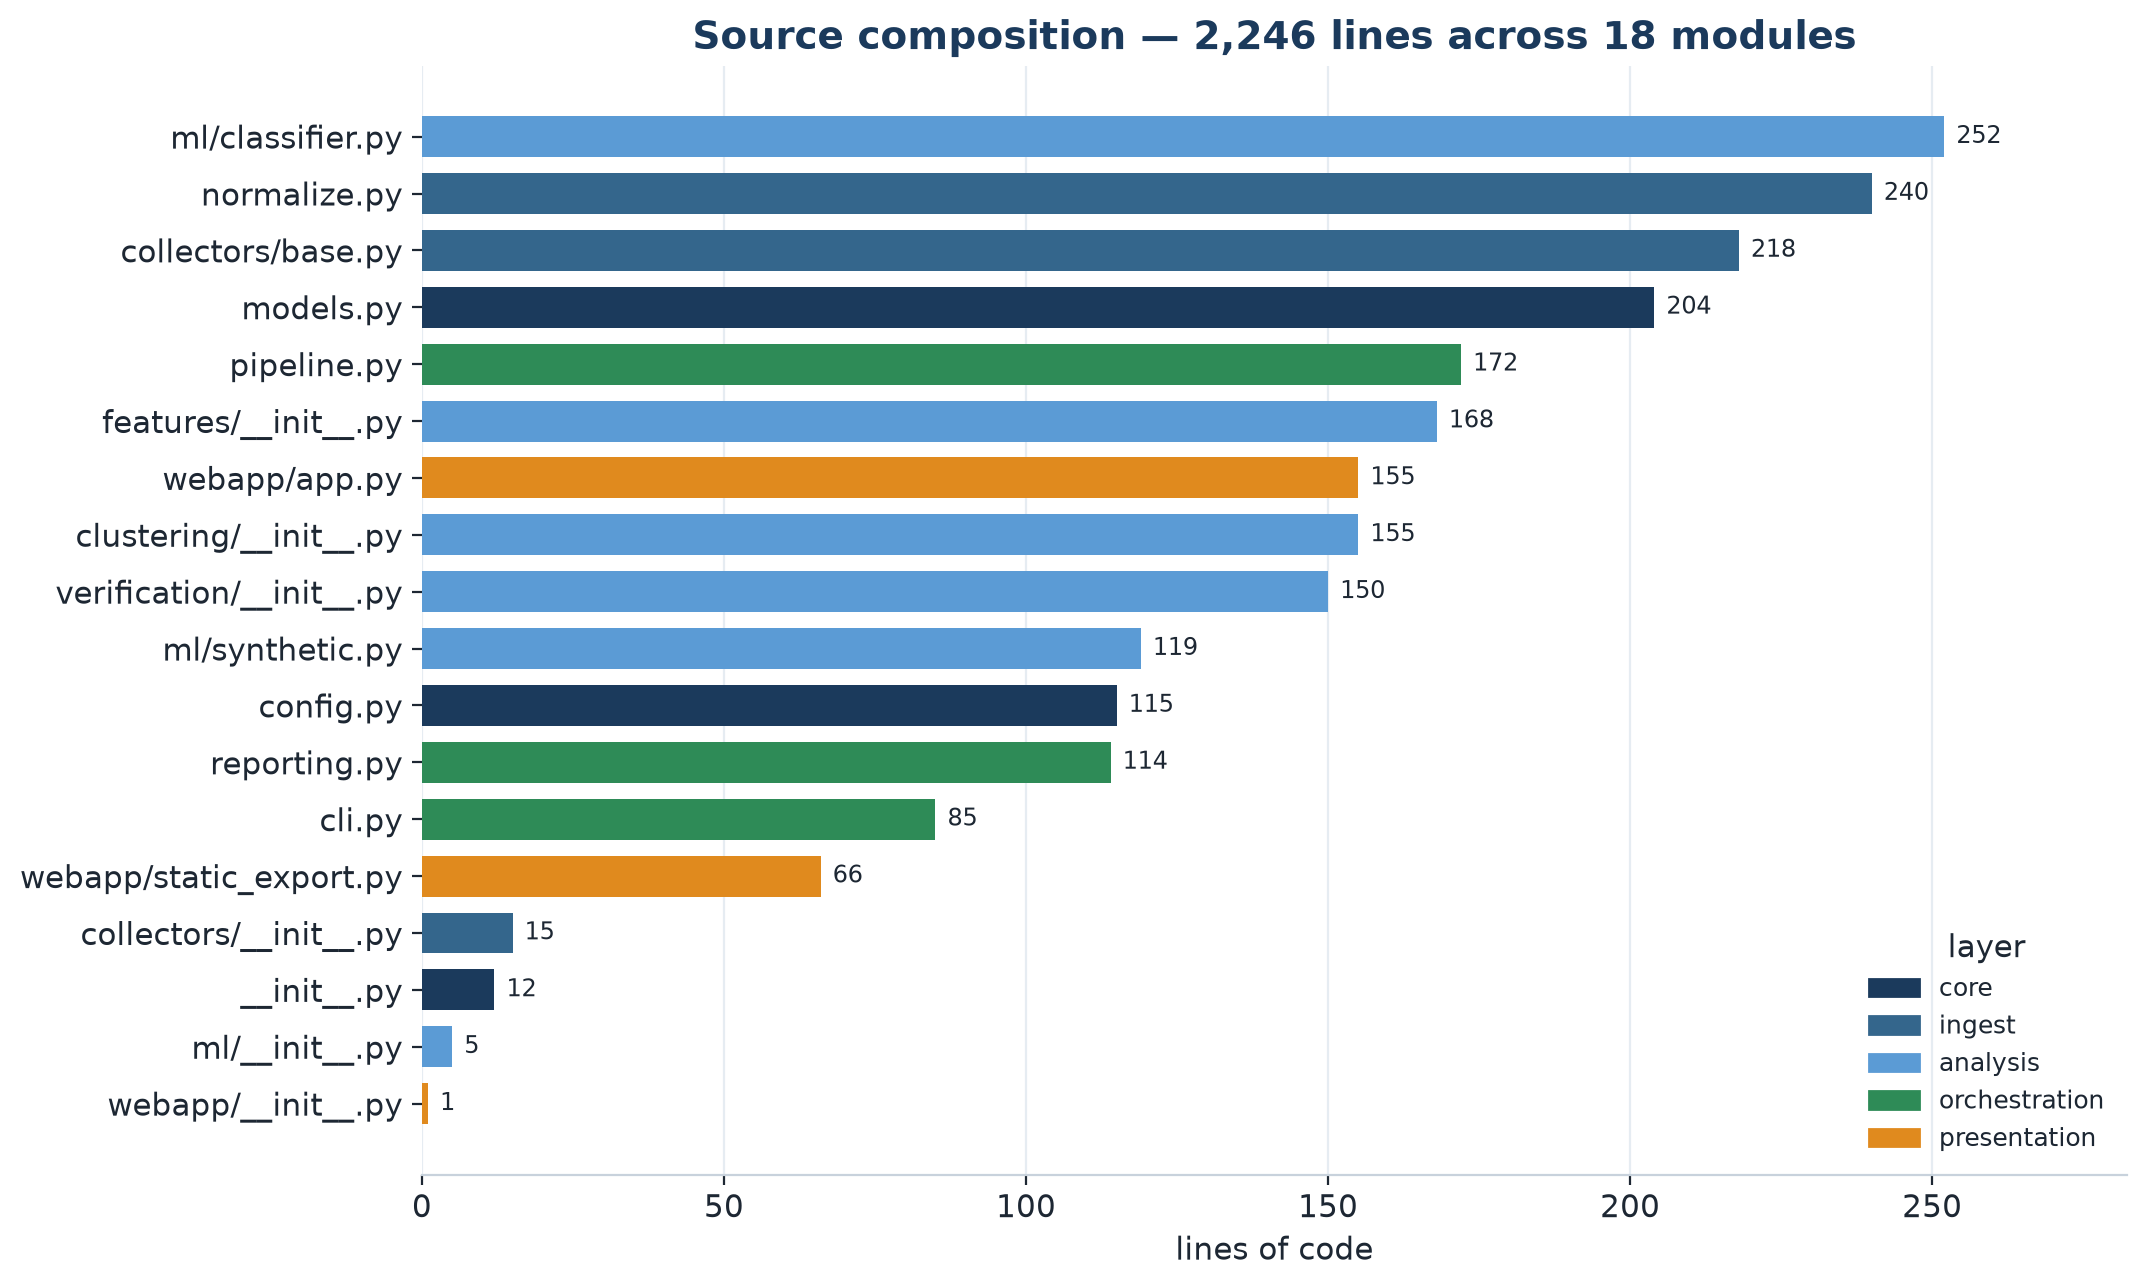
\includegraphics[width=0.92\linewidth]{figures/figB2_modules.png}
\caption{Source composition by module, coloured by architectural layer. The
analysis layer (verification, features, ML, clustering) carries the most logic;
the core data model is intentionally small.}
\label{fig:modules}
\end{figure}

Two things stand out. First, the \emph{core} layer is tiny --- \code{models.py}
and \code{config.py} together are under 320 lines --- because I kept behaviour
out of the data structures. Second, no single module exceeds 260 lines, which
kept every file small enough to hold in your head and to test in isolation.

% ============================== 8. TESTING =================================
\section{Testing strategy}

I wrote 60 tests alongside the code, not after it, and held a strict rule: test
real behaviour, not mocks. The end-to-end pipeline test runs the entire system
offline and asserts that a deliberately shared indicator is reported by at least
three sources --- an assertion that exercises collection, normalisation,
deduplication and scoring together.

\begin{figure}[htbp]
\centering
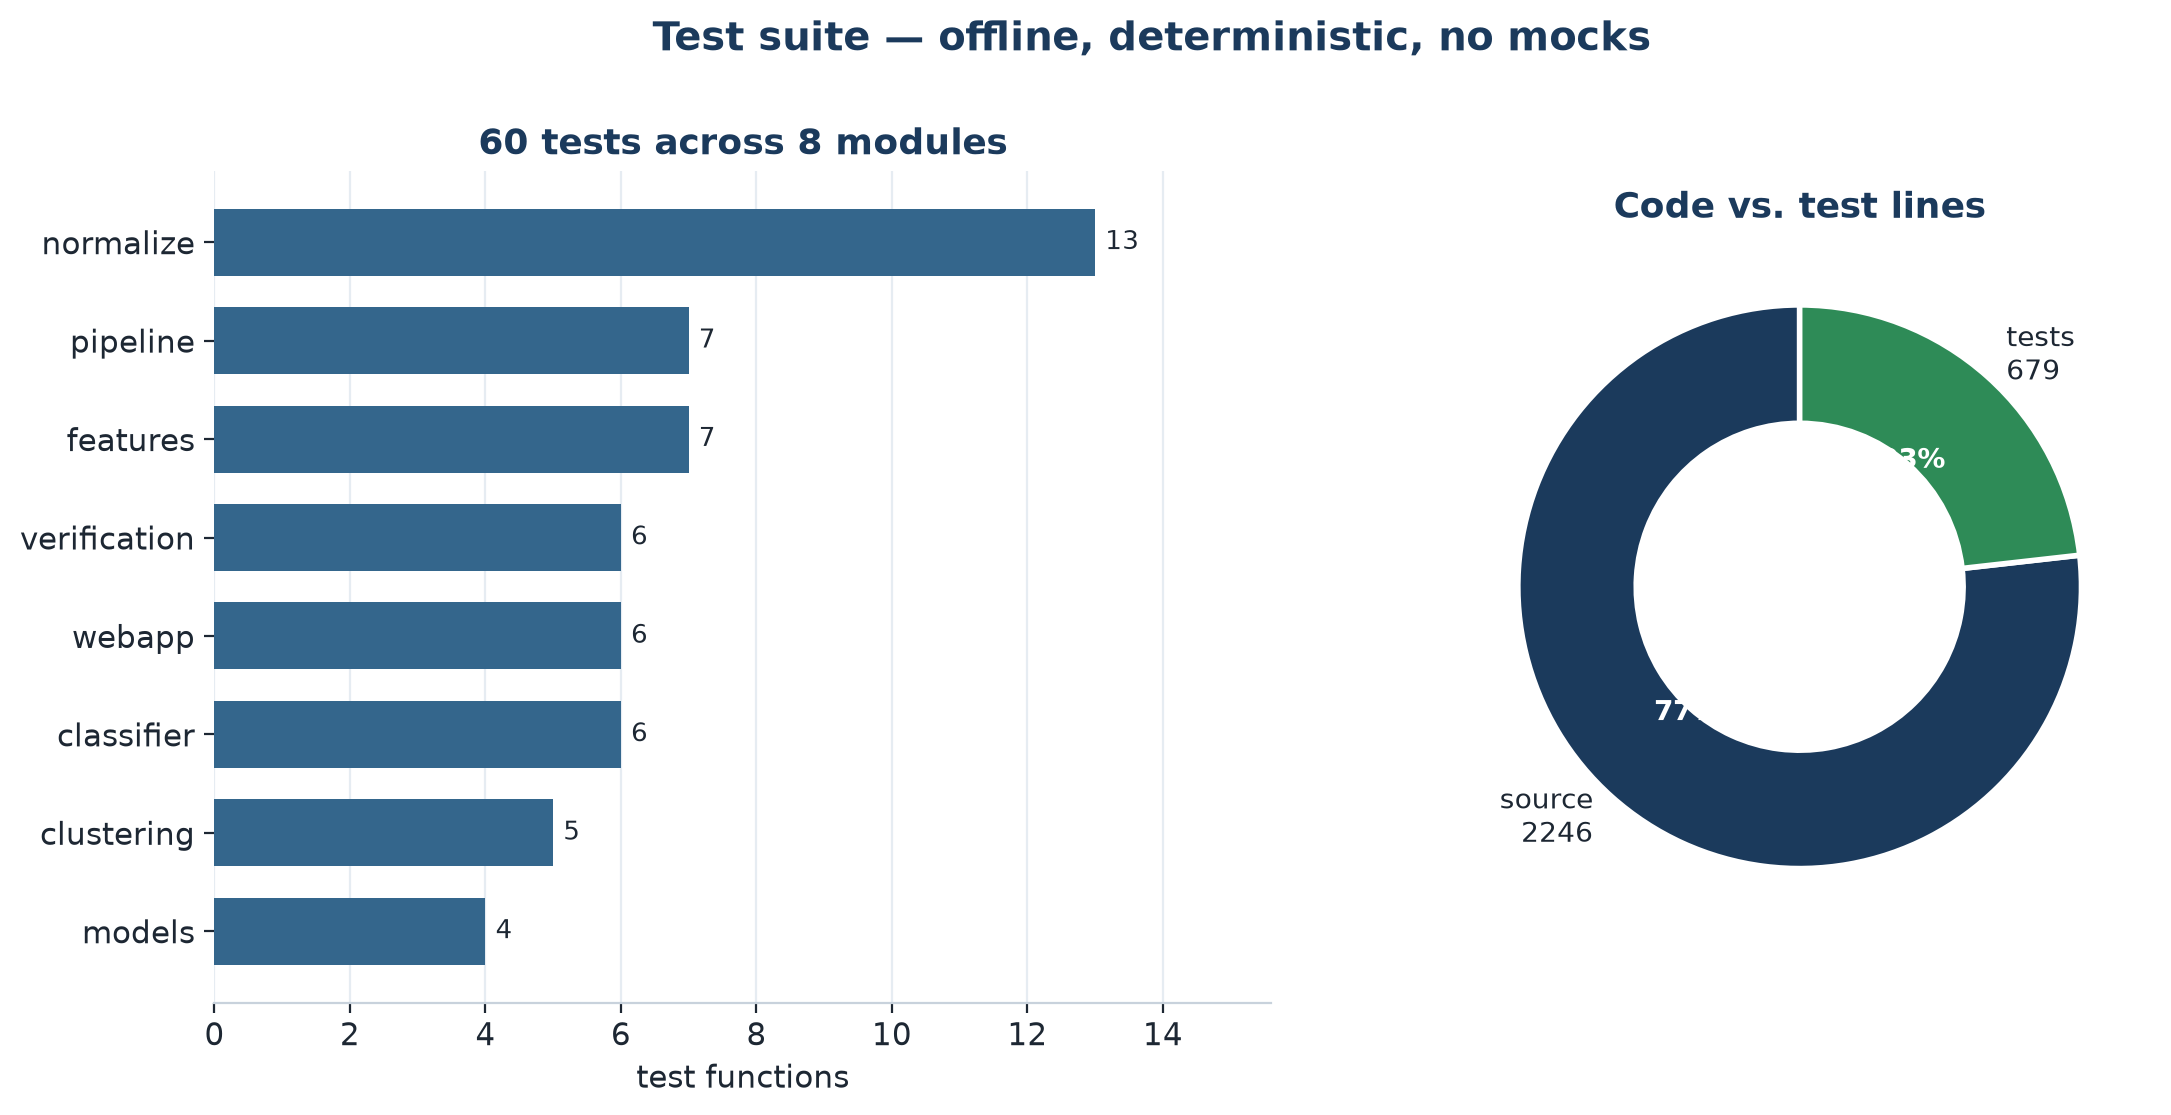
\includegraphics[width=\linewidth]{figures/figB3_tests.png}
\caption{Test distribution across modules (left) and the source-to-test line
ratio (right). Normalisation carries the most tests (13), reflecting how much
edge-case handling it contains.}
\label{fig:tests}
\end{figure}

The test-to-source ratio is roughly 1:3.3, which is a reasonable place to be for
a system whose correctness is dominated by parsing and numerical logic. Every
test is deterministic and offline --- no network, no time dependence --- so the
suite runs in under eight seconds and never flakes.

% ============================== 9. GROWTH ==================================
\section{How the codebase grew}

Figure~\ref{fig:growth} shows cumulative lines across the five commits. The
shape is informative: the first commit carries almost all of the source, and
the later commits add tests, a thin presentation layer, deployment glue and
documentation --- but barely touch the core. That is the intended shape of a
good build: heavy design up front, then additive surfaces.

\begin{figure}[htbp]
\centering
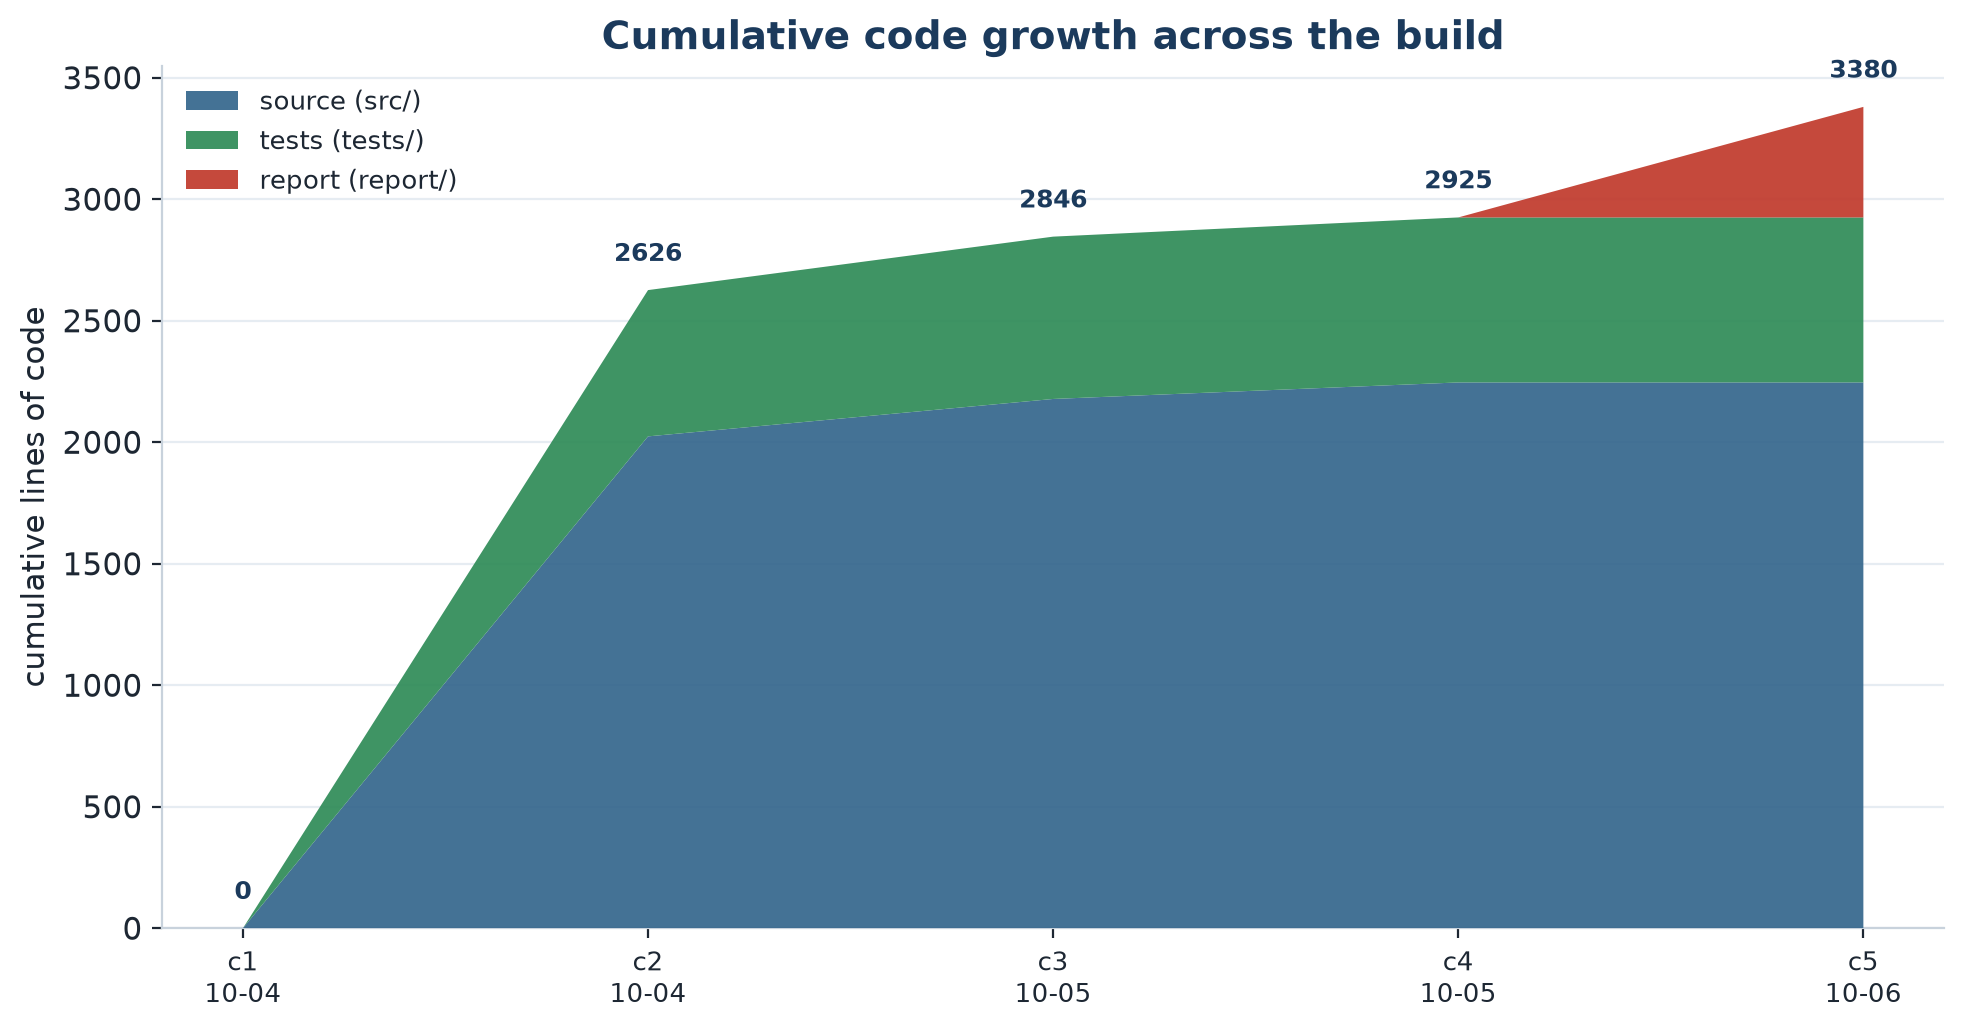
\includegraphics[width=0.95\linewidth]{figures/figB4_growth.png}
\caption{Cumulative code growth by commit, split into source, tests and report.
The core commit dominates; later work is additive.}
\label{fig:growth}
\end{figure}

% ============================== 10. STACK ==================================
\section{Technology stack}

Every dependency earns its place. There is no framework the problem did not
need, and the two heaviest (scikit-learn, Flask) are both optional extras rather
than hard requirements.

\begin{figure}[htbp]
\centering
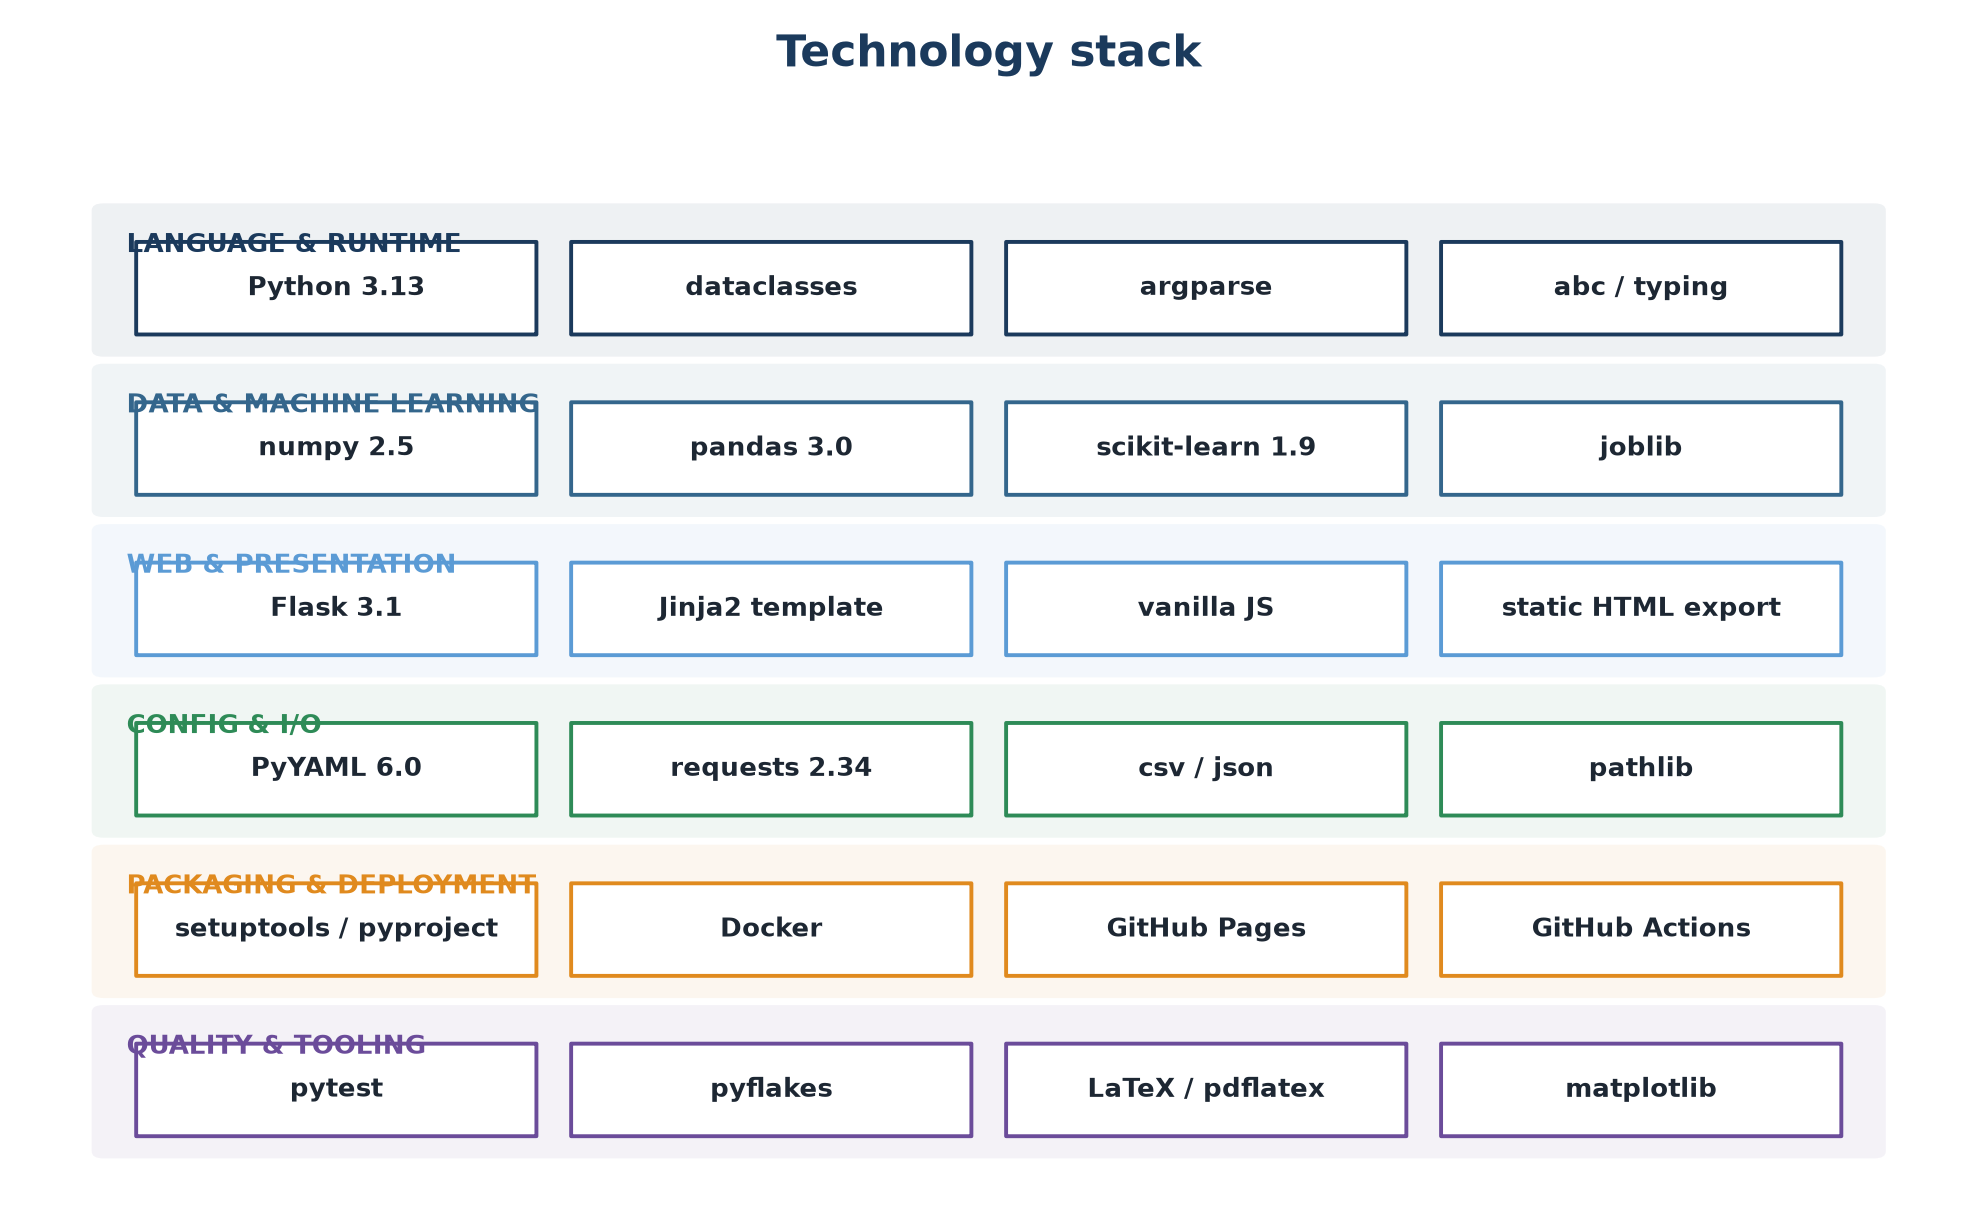
\includegraphics[width=\linewidth]{figures/figB5_stack.png}
\caption{The technology stack by layer. Core dependencies are requests, PyYAML,
numpy, pandas and scikit-learn; Flask is a \code{web} extra and pytest a
\code{dev} extra.}
\label{fig:stack}
\end{figure}

\begin{center}
\begin{tabularx}{\linewidth}{@{}>{\bfseries}p{3.6cm}>{\ttfamily}p{2.6cm}X@{}}
\toprule
\rowcolor{paper}\textbf{Choice} & \textbf{Version} & \textbf{Why this, and not something else} \\
\midrule
Language & Python 3.13 & The brief said ``bare Python 3.13''; stdlib covers hashing, CSV, config. \\
Classifier & scikit-learn 1.9 & Random forests are strong on tabular data and expose Gini importance for free --- interpretability without extra tooling. \\
Clustering & scikit-learn 1.9 & DBSCAN handles unknown cluster counts and labels outliers as noise, which is exactly right for campaigns. \\
Numeric & numpy 2.5 & Matrix work for cosine distance and the classifier input. \\
Tabular & pandas 3.0 & Convenient in analysis paths; not on the critical path. \\
Config & PyYAML 6.0 & Human-editable config with typed loading. \\
HTTP & requests 2.34 & Live feed fetching with graceful fallback. \\
Web & Flask 3.1 & Smallest thing that serves JSON and one page; no heavier framework needed. \\
Packaging & setuptools & \code{pyproject.toml} with three console scripts. \\
CI & GitHub Actions & Runs lint + tests; publishes the static dashboard. \\
Docs & LaTeX & Precise control over a metrics-heavy report with embedded figures. \\
\bottomrule
\end{tabularx}
\end{center}

% ============================== 11. WORKFLOW ===============================
\section{The workflow I followed}

Every increment went through the same loop, and I deliberately made the loop
re-runnable so verification was never optional.

\begin{figure}[htbp]
\centering
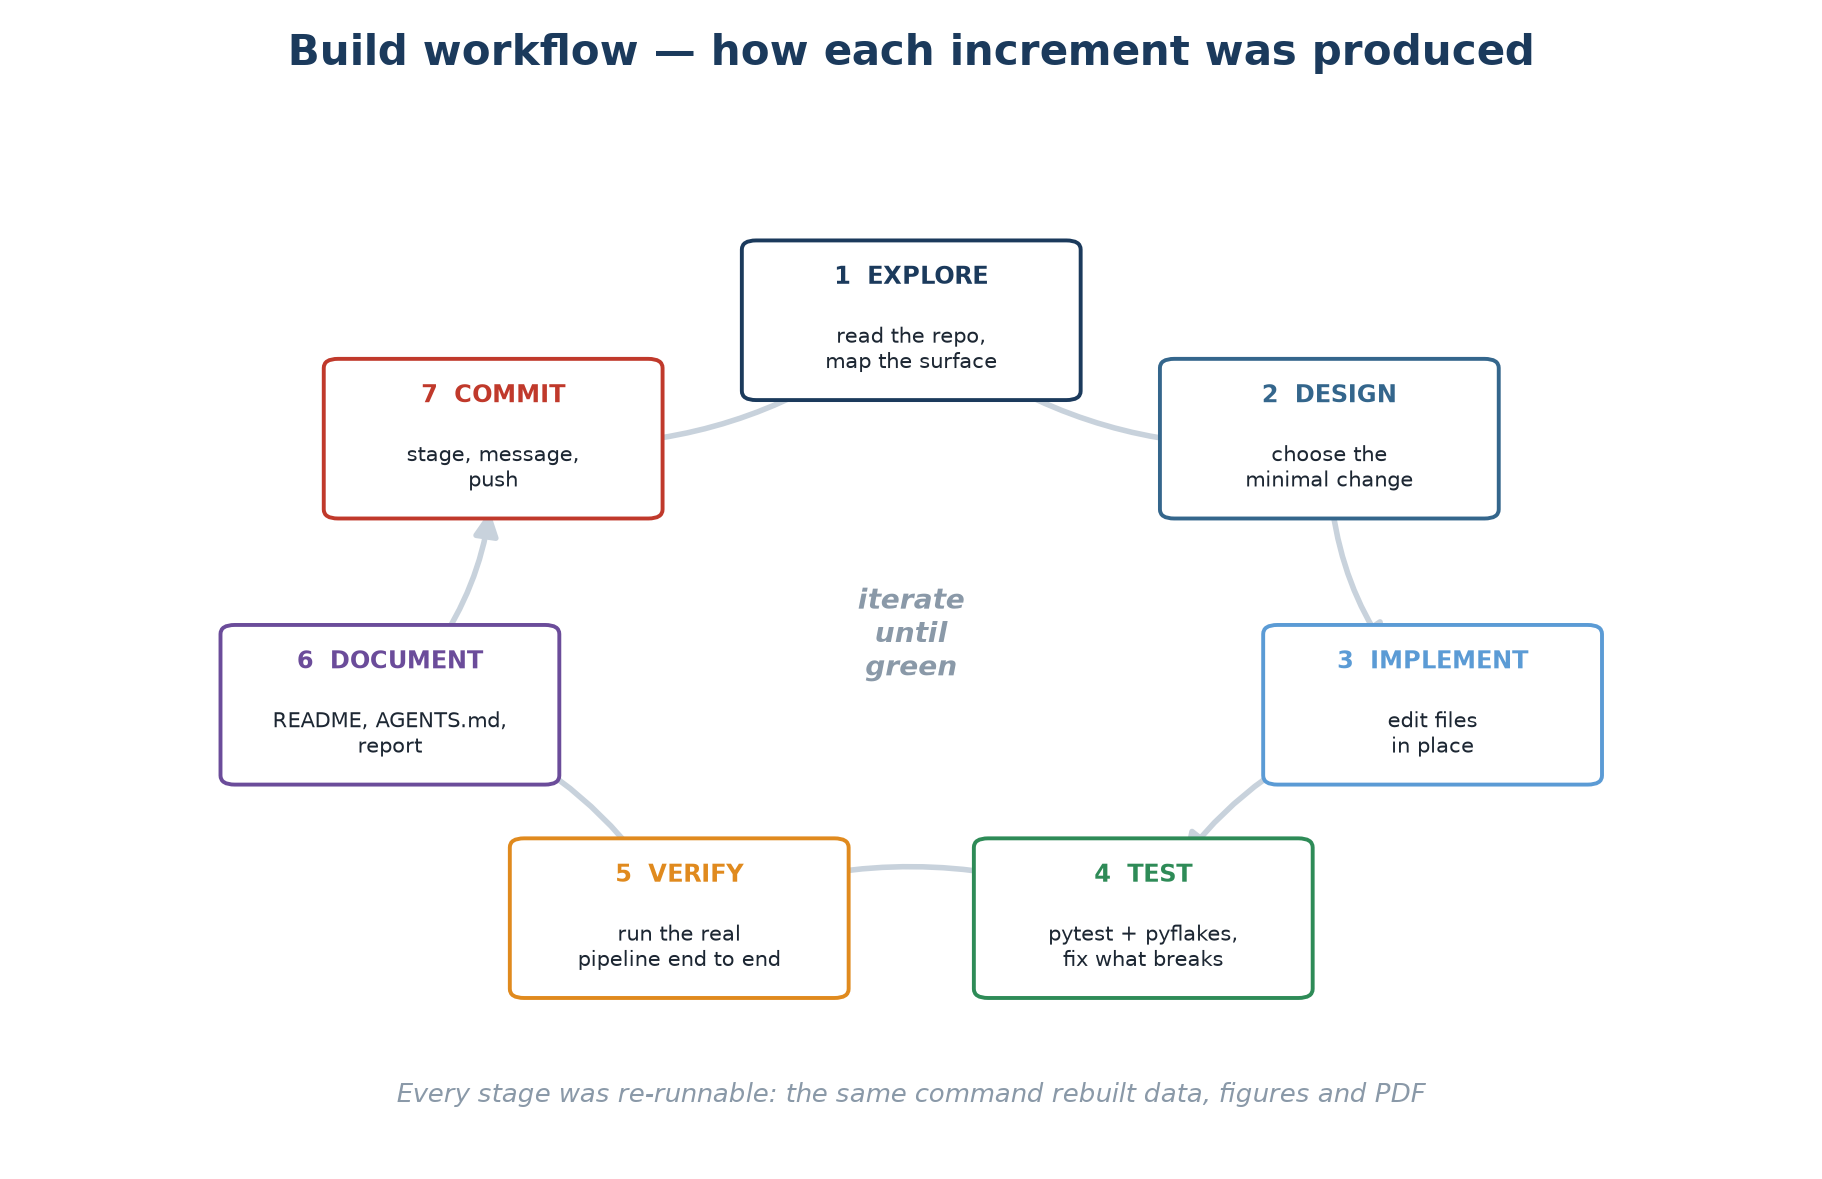
\includegraphics[width=0.82\linewidth]{figures/figB6_workflow.png}
\caption{The build loop applied to each increment. Verification (running the
real pipeline) and documentation were part of every cycle, not a final step.}
\label{fig:workflow}
\end{figure}

\begin{enumerate}[leftmargin=1.4em,itemsep=3pt]
  \item \textbf{Explore} --- read the existing tree and map the surface before
    changing anything.
  \item \textbf{Design} --- choose the \emph{minimal} change that satisfies the
    requirement, and prefer editing existing files over adding new ones.
  \item \textbf{Implement} --- write it in dependency order, keeping modules
    small.
  \item \textbf{Test} --- run \code{pytest} and \code{pyflakes}; fix what breaks
    before moving on.
  \item \textbf{Verify} --- run the \emph{real} pipeline end to end, not just the
    unit tests. This is where integration surprises surface.
  \item \textbf{Document} --- update README and AGENTS.md, and regenerate the
    report.
  \item \textbf{Commit} --- stage everything relevant with a descriptive
    message.
\end{enumerate}

% ============================== 12. OBSTACLES ==============================
\section{Obstacles and how I resolved them}

Real builds are defined by their friction. These are the genuine problems I hit,
in roughly the order I hit them, and what fixed them.

\begin{center}
\begin{tabularx}{\linewidth}{@{}>{\bfseries}p{4.6cm}X@{}}
\toprule
\rowcolor{paper}\textbf{Problem} & \textbf{Resolution} \\
\midrule
\code{pyproject.toml} had two \code{[tool.setuptools.package-data]} tables --- invalid TOML, so the package would not build & Merged the duplicate tables into one; verified with a fresh install. \\
Unused imports in \code{app.py} failed lint & Removed them; kept \code{pyflakes} clean as a gate. \\
Docker daemon present but not running & Started it manually before building; documented the requirement. \\
GitHub Pages needs a serverless artifact & Built the dual-mode template and a static exporter that inlines all data. \\
\code{pdflatex} unavailable, and \code{apt} could not find the packages & The package index was empty; ran \code{apt-get update} first, then installed TeX Live. \\
\code{matplotlib} not preinstalled & Installed it into the project virtualenv, not system-wide. \\
A tcolorbox title containing a comma broke \code{pgfkeys} & The comma is an option separator; replaced it with an em-dash. \\
Push to GitHub failed despite a valid token & The \emph{remote URL} still embedded an old, expired token. Refreshed the remote URL with the current token and pushed. \\
Could not visually inspect figures through the browser & Fell back to \code{pdftotext}/\code{pdftoppm} to extract and render pages for verification. \\
\bottomrule
\end{tabularx}
\end{center}

\begin{warstory}[The one that mattered most: a stale token in the remote]
The push had been ``blocked by an expired GitHub token'' across sessions. When I
finally probed the API directly, the token authenticated fine --- it was the
\emph{git remote URL} that still carried an old credential baked in at clone
time. Updating the remote with the current token fixed a blocker that had
looked like an auth problem for days. The lesson: when authentication ``fails,''
check \emph{every} place the credential is stored, not just the one you are
thinking about.
\end{warstory}

% ============================== 13. QUALITY ================================
\section{Quality at a glance}

\begin{figure}[htbp]
\centering
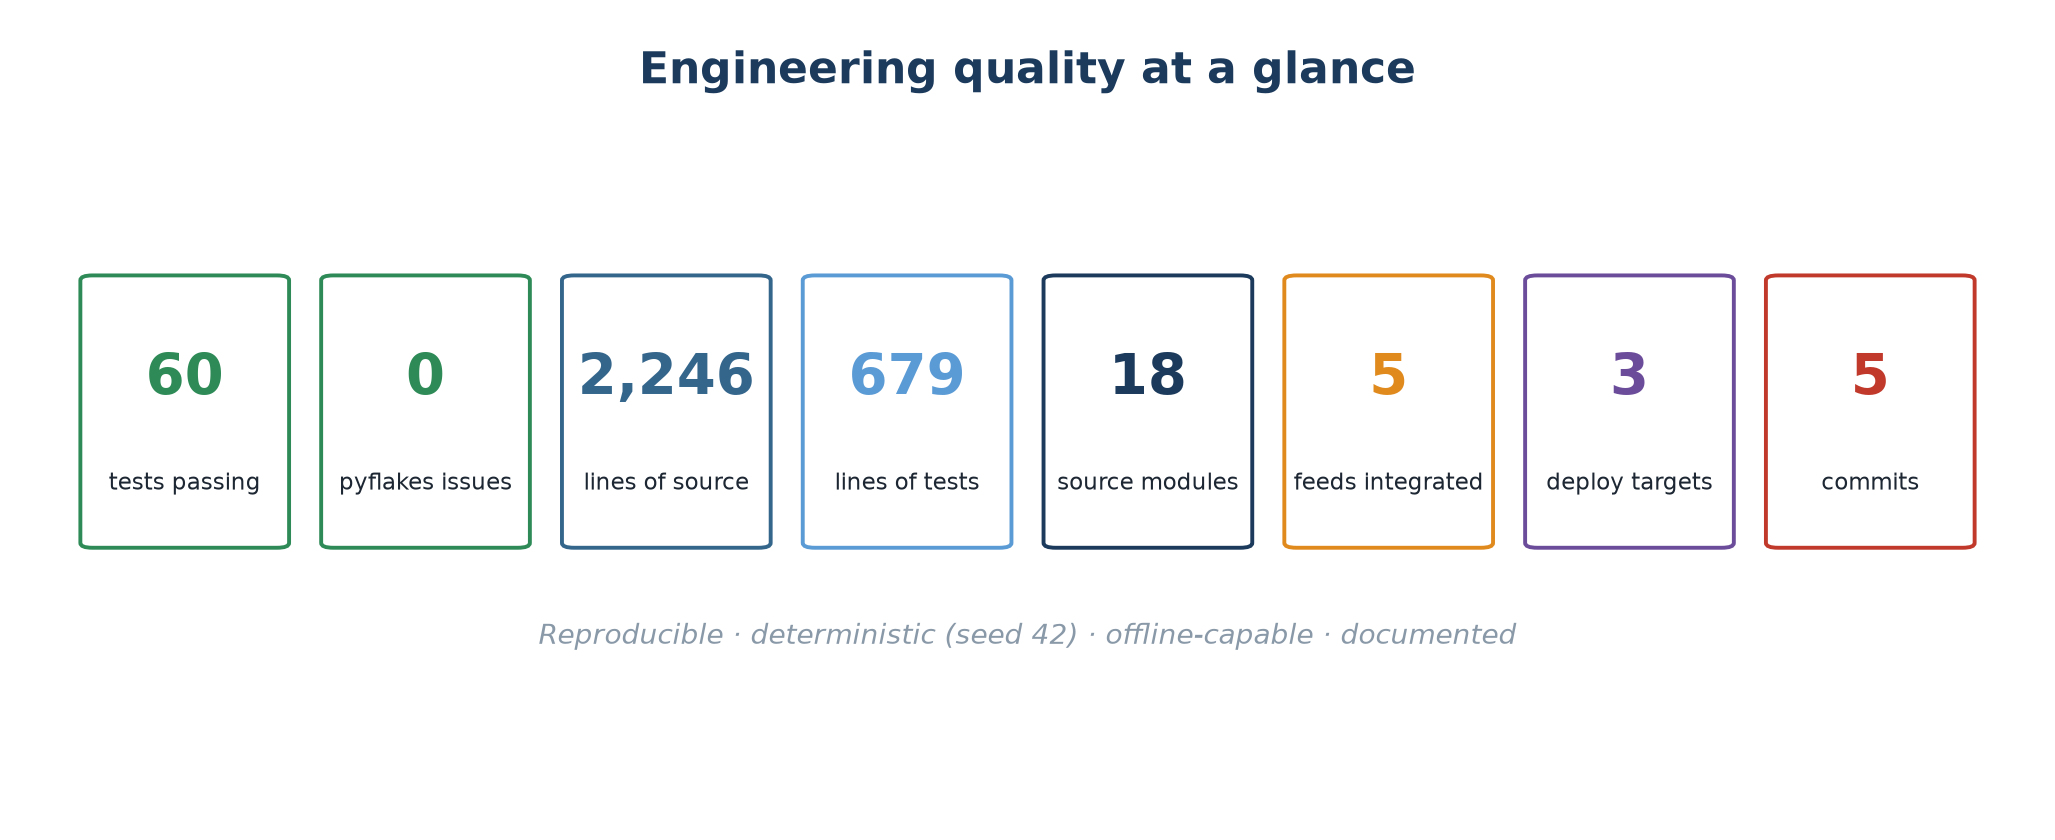
\includegraphics[width=\linewidth]{figures/figB7_quality.png}
\caption{Final engineering metrics for the build.}
\label{fig:quality}
\end{figure}

\begin{keybox}[Verified state of the repository]
\begin{tabularx}{\linewidth}{@{}lX@{}}
\textbf{Tests} & 60 passing, offline and deterministic, in under 8\,s \\
\textbf{Lint} & \code{pyflakes} clean across source, tests and report scripts \\
\textbf{Source} & 2{,}246 lines across 18 modules \\
\textbf{Tests} & 679 lines across 8 test modules \\
\textbf{Deployment} & GitHub Pages, Docker and CI --- all exercised locally \\
\textbf{Reproducibility} & one seed; \code{build\_report.sh} rebuilds data, figures and PDF \\
\end{tabularx}
\end{keybox}

% ============================== 14. RETROSPECTIVE ==========================
\section{Retrospective}

\subsection{What went well}
\begin{itemize}[leftmargin=1.4em,itemsep=3pt]
  \item \textbf{Data model first.} Defining the five dataclasses before any
    logic kept every module decoupled and made the pipeline a readable sequence
    of transforms.
  \item \textbf{Offline-first.} Fixtures and graceful fallback gave me
    determinism, CI-friendliness and real-world resilience in one decision.
  \item \textbf{Generated documentation.} Because figures come from pipeline
    output, the report cannot silently drift from the code.
  \item \textbf{Small modules.} Nothing exceeded 260 lines; everything stayed
    testable in isolation.
\end{itemize}

\subsection{What I would do differently}
\begin{itemize}[leftmargin=1.4em,itemsep=3pt]
  \item \textbf{Check credentials in all locations sooner.} The stale-token
    blocker cost time because I trusted the error message's framing.
  \item \textbf{Add a live smoke test earlier.} The 403-on-one-feed behaviour
    was discovered late; a scheduled live run would have surfaced it sooner.
  \item \textbf{Parameterise the clustering distance.} The 0.6/0.4 lexical-to-tag
    weighting is principled but hand-set; it deserves a small tuning harness.
  \item \textbf{Broader Python matrix in CI.} I test 3.10 and 3.12; 3.13 (the
    actual target) should be in the matrix.
\end{itemize}

\subsection{What comes next}
The system is a foundation, and the path forward is mostly about \emph{data}, not
architecture: point \code{--labels} at analyst-reviewed ground truth, widen the
corpus, add temporal decay to source reliability, and model shared
infrastructure as a graph to link campaigns beyond lexical similarity. None of
those require redesign --- the seams are already in place.

% ============================== 15. CONCLUSION =============================
\section{Conclusion}

ThreatInt went from a three-line README to a tested, deployed, documented
pipeline in five commits and three days. The build was not defined by exotic
algorithms but by a handful of disciplined choices made early and held
consistently: put the data model first, make the offline path real, compute trust
instead of assuming it, keep modules small, and generate documentation from the
code rather than beside it.

The friction was real --- invalid TOML, a dormant Docker daemon, an empty
package index, a LaTeX option-parsing quirk, and a credential that turned out to
be stale in the one place I was not looking. Each was small; together they are
the honest texture of shipping software. Recording them here is the point of a
build report: the technical research report explains what the system \emph{is};
this document explains how it came to be, and what that process taught me.

\vspace{0.5cm}
\begin{center}
\rule{8cm}{0.4pt}\\[0.25cm]
{\footnotesize\color{grey}
ThreatInt v0.1.0 · Engineering Build Report · companion to the Technical
Research Report}
\end{center}

\end{document}
